% !TEX program = xelatex
% P/D 比率上升的来源：数据否定分红坍缩，指向资金侧。主窗口 2009–2025（u 态），2009 之前仅作灰色背景。Calibration R1 检查阶段，2026-11-13。
% 图：figures/*.pdf（scripts/build_data.py 生成）；数值：data/values.tex（同一脚本生成，\val{key}）。颜色：蓝=数据，橙=模型，绿=Compustat 队列，灰=2009 之前。
\documentclass[aspectratio=169,10pt]{beamer}
\usepackage{xeCJK}
\setCJKmainfont{Hiragino Sans GB}
\setCJKsansfont{Hiragino Sans GB}
\xeCJKsetup{PunctStyle=kaiming}
\usepackage{amsmath,amssymb,booktabs,graphicx,array,xcolor}
\usetheme{default}
\setbeamertemplate{navigation symbols}{}
\setbeamertemplate{footline}{\hfill\textcolor{muted}{\scriptsize\insertframenumber}\hspace{0.4cm}\vspace{0.25cm}}
\setbeamertemplate{itemize items}[circle]
\setbeamertemplate{frametitle}{\vspace{0.45cm}\textbf{\large\insertframetitle}\\[-0.05cm]{\small\textcolor{inksec}{\insertframesubtitle}}\vspace{0.1cm}}
\definecolor{ink}{HTML}{0B0B0B}\definecolor{inksec}{HTML}{52514E}\definecolor{muted}{HTML}{898781}
\definecolor{dataC}{HTML}{2A78D6}\definecolor{dataD}{HTML}{104281}\definecolor{modelC}{HTML}{EB6834}\definecolor{greenC}{HTML}{1BAF7A}\definecolor{washc}{HTML}{F0EFEC}\definecolor{ctxc}{HTML}{C3C2B7}
\setbeamercolor{normal text}{fg=ink,bg=white}\setbeamercolor{structure}{fg=dataD}\setbeamercolor{frametitle}{fg=ink}
\setbeamercolor{block title}{fg=white,bg=dataD}\setbeamercolor{block body}{fg=ink,bg=washc}
\setlength{\leftmargini}{1.1em}
\newcommand{\val}[1]{\csname v:#1\endcsname}
% generated by build_data.py; use \val{key} in the deck
\expandafter\def\csname v:multQ\endcsname{5.5}
\expandafter\def\csname v:grQ\endcsname{11.2}
\expandafter\def\csname v:multBQ\endcsname{4.3}
\expandafter\def\csname v:grBQ\endcsname{10.9}
\expandafter\def\csname v:multFCF\endcsname{1.99}
\expandafter\def\csname v:grFCF\endcsname{4.4}
\expandafter\def\csname v:multBFCF\endcsname{2.1}
\expandafter\def\csname v:grBFCF\endcsname{5.4}
\expandafter\def\csname v:multY\endcsname{2.3}
\expandafter\def\csname v:grY\endcsname{5.3}
\expandafter\def\csname v:multBY\endcsname{2.1}
\expandafter\def\csname v:grBY\endcsname{5.3}
\expandafter\def\csname v:multCOMP\endcsname{2.2}
\expandafter\def\csname v:grCOMP\endcsname{4.9}
\expandafter\def\csname v:multBCOMP\endcsname{2.0}
\expandafter\def\csname v:grBCOMP\endcsname{5.1}
\expandafter\def\csname v:gapDe09\endcsname{-0.52}
\expandafter\def\csname v:gapDe11\endcsname{0.28}
\expandafter\def\csname v:Demin\endcsname{18.4}
\expandafter\def\csname v:Demax\endcsname{26.3}
\expandafter\def\csname v:D_Q2009\endcsname{7.4}
\expandafter\def\csname v:CASHDIV_EQ2009\endcsname{5.5}
\expandafter\def\csname v:D_e2009\endcsname{24.5}
\expandafter\def\csname v:D_Y2009\endcsname{14.4}
\expandafter\def\csname v:PROFIT_SHARE2009\endcsname{41.1}
\expandafter\def\csname v:Q_e2009\endcsname{3.3}
\expandafter\def\csname v:A_e2009\endcsname{2.7}
\expandafter\def\csname v:Q_Y2009\endcsname{1.94}
\expandafter\def\csname v:EL_Y_sept2009\endcsname{0.69}
\expandafter\def\csname v:D_Q2010\endcsname{5.9}
\expandafter\def\csname v:CASHDIV_EQ2010\endcsname{4.9}
\expandafter\def\csname v:D_e2010\endcsname{23.8}
\expandafter\def\csname v:D_Y2010\endcsname{13.6}
\expandafter\def\csname v:PROFIT_SHARE2010\endcsname{42.9}
\expandafter\def\csname v:Q_e2010\endcsname{4.1}
\expandafter\def\csname v:A_e2010\endcsname{3.5}
\expandafter\def\csname v:Q_Y2010\endcsname{2.3}
\expandafter\def\csname v:EL_Y_sept2010\endcsname{0.78}
\expandafter\def\csname v:D_Q2011\endcsname{5.5}
\expandafter\def\csname v:CASHDIV_EQ2011\endcsname{5.5}
\expandafter\def\csname v:D_e2011\endcsname{21.8}
\expandafter\def\csname v:D_Y2011\endcsname{12.5}
\expandafter\def\csname v:PROFIT_SHARE2011\endcsname{42.6}
\expandafter\def\csname v:Q_e2011\endcsname{3.9}
\expandafter\def\csname v:A_e2011\endcsname{3.1}
\expandafter\def\csname v:Q_Y2011\endcsname{2.3}
\expandafter\def\csname v:EL_Y_sept2011\endcsname{0.79}
\expandafter\def\csname v:D_Q2013\endcsname{3.8}
\expandafter\def\csname v:CASHDIV_EQ2013\endcsname{4.9}
\expandafter\def\csname v:D_e2013\endcsname{20.2}
\expandafter\def\csname v:D_Y2013\endcsname{11.5}
\expandafter\def\csname v:PROFIT_SHARE2013\endcsname{43.1}
\expandafter\def\csname v:Q_e2013\endcsname{5.3}
\expandafter\def\csname v:A_e2013\endcsname{4.3}
\expandafter\def\csname v:Q_Y2013\endcsname{3.0}
\expandafter\def\csname v:EL_Y_sept2013\endcsname{1.08}
\expandafter\def\csname v:D_Q2015\endcsname{3.4}
\expandafter\def\csname v:CASHDIV_EQ2015\endcsname{5.1}
\expandafter\def\csname v:D_e2015\endcsname{18.4}
\expandafter\def\csname v:D_Y2015\endcsname{10.5}
\expandafter\def\csname v:PROFIT_SHARE2015\endcsname{42.9}
\expandafter\def\csname v:Q_e2015\endcsname{5.3}
\expandafter\def\csname v:A_e2015\endcsname{4.1}
\expandafter\def\csname v:Q_Y2015\endcsname{3.0}
\expandafter\def\csname v:EL_Y_sept2015\endcsname{1.07}
\expandafter\def\csname v:D_Q2019\endcsname{3.1}
\expandafter\def\csname v:CASHDIV_EQ2019\endcsname{4.1}
\expandafter\def\csname v:D_e2019\endcsname{19.6}
\expandafter\def\csname v:D_Y2019\endcsname{11.4}
\expandafter\def\csname v:PROFIT_SHARE2019\endcsname{42.0}
\expandafter\def\csname v:Q_e2019\endcsname{6.2}
\expandafter\def\csname v:A_e2019\endcsname{4.7}
\expandafter\def\csname v:Q_Y2019\endcsname{3.6}
\expandafter\def\csname v:EL_Y_sept2019\endcsname{1.46}
\expandafter\def\csname v:D_Q2025\endcsname{2.7}
\expandafter\def\csname v:CASHDIV_EQ2025\endcsname{2.7}
\expandafter\def\csname v:D_e2025\endcsname{22.6}
\expandafter\def\csname v:D_Y2025\endcsname{12.7}
\expandafter\def\csname v:PROFIT_SHARE2025\endcsname{44.1}
\expandafter\def\csname v:Q_e2025\endcsname{8.3}
\expandafter\def\csname v:A_e2025\endcsname{6.3}
\expandafter\def\csname v:Q_Y2025\endcsname{4.7}
\expandafter\def\csname v:EL_Y_sept2025\endcsname{1.94}
\expandafter\def\csname v:ELYmult\endcsname{2.8}
\expandafter\def\csname v:DYmult\endcsname{0.88}
\expandafter\def\csname v:eYmult\endcsname{0.95}
\expandafter\def\csname v:ELYmult11\endcsname{2.5}
\expandafter\def\csname v:DYmult11\endcsname{1.01}
\expandafter\def\csname v:decQD2009\endcsname{1.01}
\expandafter\def\csname v:decQY2009\endcsname{0.88}
\expandafter\def\csname v:decDY2009\endcsname{0.13}
\expandafter\def\csname v:decShare2009\endcsname{87.0}
\expandafter\def\csname v:decQD2011\endcsname{0.71}
\expandafter\def\csname v:decQY2011\endcsname{0.72}
\expandafter\def\csname v:decDY2011\endcsname{-0.01}
\expandafter\def\csname v:decShare2011\endcsname{102}
\expandafter\def\csname v:decQD2013\endcsname{0.33}
\expandafter\def\csname v:decQY2013\endcsname{0.43}
\expandafter\def\csname v:decDY2013\endcsname{-0.10}
\expandafter\def\csname v:decShare2013\endcsname{130}
\expandafter\def\csname v:aSlope\endcsname{-7.0}
\expandafter\def\csname v:aIdx2022\endcsname{0.42}
\expandafter\def\csname v:QwH0922\endcsname{2.4}
\expandafter\def\csname v:BHQ2009\endcsname{0.12}
\expandafter\def\csname v:BHQ2022\endcsname{0.08}
\expandafter\def\csname v:Hmult\endcsname{1.61}
\expandafter\def\csname v:Hgr\endcsname{3.2}
\expandafter\def\csname v:nscg2010\endcsname{6.9}
\expandafter\def\csname v:nscg2023\endcsname{7.3}
\expandafter\def\csname v:lccps2015\endcsname{8.3}
\expandafter\def\csname v:lccps2023\endcsname{10.5}
\expandafter\def\csname v:reqA2009\endcsname{66.1}
\expandafter\def\csname v:reqB2009\endcsname{17.1}
\expandafter\def\csname v:reqA2010\endcsname{57.1}
\expandafter\def\csname v:reqB2010\endcsname{14.0}
\expandafter\def\csname v:reqA2011\endcsname{54.3}
\expandafter\def\csname v:reqB2011\endcsname{13.3}
\expandafter\def\csname v:reqA2013\endcsname{33.4}
\expandafter\def\csname v:reqB2013\endcsname{9.5}
\expandafter\def\csname v:reqA2015\endcsname{26.8}
\expandafter\def\csname v:reqB2015\endcsname{8.7}
\expandafter\def\csname v:BHQ2010\endcsname{0.10}
\expandafter\def\csname v:G07_2010\endcsname{0.72}
\expandafter\def\csname v:mu07_2010\endcsname{1.62}
\expandafter\def\csname v:BHQ2013\endcsname{0.08}
\expandafter\def\csname v:G07_2013\endcsname{0.58}
\expandafter\def\csname v:mu07_2013\endcsname{1.49}
\expandafter\def\csname v:BHQ2015\endcsname{0.08}
\expandafter\def\csname v:G07_2015\endcsname{0.59}
\expandafter\def\csname v:mu07_2015\endcsname{1.44}
\expandafter\def\csname v:BHQ2019\endcsname{0.08}
\expandafter\def\csname v:G07_2019\endcsname{0.54}
\expandafter\def\csname v:mu07_2019\endcsname{1.44}
\expandafter\def\csname v:G07_2022\endcsname{0.56}
\expandafter\def\csname v:mu07_2022\endcsname{1.46}
\expandafter\def\csname v:BHQ2024\endcsname{0.06}
\expandafter\def\csname v:G07_2024\endcsname{0.45}
\expandafter\def\csname v:mu07_2024\endcsname{1.48}
\expandafter\def\csname v:Gmin\endcsname{0.32}
\expandafter\def\csname v:Gmax\endcsname{0.85}
\expandafter\def\csname v:mumin\endcsname{1.43}
\expandafter\def\csname v:mumax\endcsname{1.51}
\expandafter\def\csname v:c2009dvt_mult\endcsname{2.3}
\expandafter\def\csname v:c2009netpay_mult\endcsname{7.9}
\expandafter\def\csname v:c2009fcf_mult\endcsname{1.50}
\expandafter\def\csname v:c2009me_mult\endcsname{3.9}
\expandafter\def\csname v:c2009comp_mult\endcsname{2.1}
\expandafter\def\csname v:c2009Q_ahp_mult\endcsname{5.0}
\expandafter\def\csname v:c2009all_dvt_mult\endcsname{2.6}
\expandafter\def\csname v:c2009all_me_mult\endcsname{5.0}
\expandafter\def\csname v:c2009n0\endcsname{6,146}
\expandafter\def\csname v:c2009n2024\endcsname{2,361}
\expandafter\def\csname v:c2009dvt_gr\endcsname{5.8}
\expandafter\def\csname v:c2009netpay_gr\endcsname{14.7}
\expandafter\def\csname v:c2009comp_gr\endcsname{4.9}
\expandafter\def\csname v:c2009me_gr\endcsname{9.6}
\expandafter\def\csname v:c2009dvt_me0\endcsname{2.6}
\expandafter\def\csname v:c2009dvt_me2024\endcsname{1.54}
\expandafter\def\csname v:c2009share_dvt2024\endcsname{89.7}
\expandafter\def\csname v:c2009share_me2024\endcsname{73.3}
\expandafter\def\csname v:c2010dvt_mult\endcsname{2.3}
\expandafter\def\csname v:c2010netpay_mult\endcsname{3.8}
\expandafter\def\csname v:c2010fcf_mult\endcsname{1.40}
\expandafter\def\csname v:c2010me_mult\endcsname{3.6}
\expandafter\def\csname v:c2010comp_mult\endcsname{2.0}
\expandafter\def\csname v:c2010Q_ahp_mult\endcsname{3.9}
\expandafter\def\csname v:c2010all_dvt_mult\endcsname{2.4}
\expandafter\def\csname v:c2010all_me_mult\endcsname{4.3}
\expandafter\def\csname v:c2010n0\endcsname{6,033}
\expandafter\def\csname v:c2010n2024\endcsname{2,483}
\expandafter\def\csname v:c2010dvt_gr\endcsname{6.0}
\expandafter\def\csname v:c2010netpay_gr\endcsname{9.9}
\expandafter\def\csname v:c2010comp_gr\endcsname{5.1}
\expandafter\def\csname v:c2010me_gr\endcsname{9.5}
\expandafter\def\csname v:c2010dvt_me0\endcsname{2.4}
\expandafter\def\csname v:c2010dvt_me2024\endcsname{1.52}
\expandafter\def\csname v:c2010share_dvt2024\endcsname{93.3}
\expandafter\def\csname v:c2010share_me2024\endcsname{77.0}
\expandafter\def\csname v:c2011dvt_mult\endcsname{2.00}
\expandafter\def\csname v:c2011netpay_mult\endcsname{2.5}
\expandafter\def\csname v:c2011fcf_mult\endcsname{1.28}
\expandafter\def\csname v:c2011me_mult\endcsname{3.6}
\expandafter\def\csname v:c2011comp_mult\endcsname{1.92}
\expandafter\def\csname v:c2011Q_ahp_mult\endcsname{3.8}
\expandafter\def\csname v:c2011all_dvt_mult\endcsname{2.1}
\expandafter\def\csname v:c2011all_me_mult\endcsname{4.3}
\expandafter\def\csname v:c2011n0\endcsname{6,002}
\expandafter\def\csname v:c2011n2024\endcsname{2,605}
\expandafter\def\csname v:c2011dvt_gr\endcsname{5.5}
\expandafter\def\csname v:c2011netpay_gr\endcsname{7.1}
\expandafter\def\csname v:c2011comp_gr\endcsname{5.2}
\expandafter\def\csname v:c2011me_gr\endcsname{10.4}
\expandafter\def\csname v:c2011dvt_me0\endcsname{2.8}
\expandafter\def\csname v:c2011dvt_me2024\endcsname{1.52}
\expandafter\def\csname v:c2011share_dvt2024\endcsname{93.8}
\expandafter\def\csname v:c2011share_me2024\endcsname{77.6}
\expandafter\def\csname v:allNlisted2009\endcsname{4,457}
\expandafter\def\csname v:allNlisted2024\endcsname{5,028}
\expandafter\def\csname v:allNlistedMin\endcsname{4,399}
\expandafter\def\csname v:allNlistedMinYear\endcsname{2,012}
\expandafter\def\csname v:netissMean\endcsname{-1.08}
\expandafter\def\csname v:netissNegYears\endcsname{15}
\expandafter\def\csname v:netissYears\endcsname{16}
\expandafter\def\csname v:buyback2024\endcsname{1,116}
\expandafter\def\csname v:issue2024\endcsname{346}
\expandafter\def\csname v:buybackCum\endcsname{11.4}
\expandafter\def\csname v:issueCum\endcsname{5.1}
\expandafter\def\csname v:allDvtMe2009\endcsname{2.4}
\expandafter\def\csname v:allDvtMe2024\endcsname{1.26}
\expandafter\def\csname v:allMeMult\endcsname{5.0}

\newcommand{\src}[1]{\vfill{\scriptsize\textcolor{muted}{#1}}}
\newcommand{\en}[1]{\textcolor{inksec}{#1}}
\hypersetup{pdftitle={P/D ratio 2009-2025: alternatives to the R&D-share channel},colorlinks=true,urlcolor=dataD,linkcolor=ink}

\begin{document}

% ---------------------------------------------------------------- 1
\begin{frame}[plain]
\vspace{1.2cm}
{\scriptsize\textcolor{muted}{\textbf{CALIBRATION R1, CHECK PHASE}}}\\[0.3cm]
{\Large\textbf{P/D 比率上升的来源：数据否定分红坍缩，指向资金侧}}\\[0.35cm]
{\normalsize\textcolor{inksec}{Alternative mechanisms for an explosive price-dividend ratio when the R\&D labor share does not go to one. 主窗口 2009 到 2025 年，即 unbalanced-growth 态；2009 之前只作灰色背景。}}\\[0.6cm]
\begin{columns}[T]
\column{0.46\textwidth}
{\small\textbf{图例}}\\[0.15cm]
{\small\textcolor{dataC}{\rule{1cm}{2.2pt}}\; 数据 \en{(data)}\quad \textcolor{modelC}{\rule{1cm}{2.2pt}}\; 模型 \en{(model)}\quad \textcolor{greenC}{\rule{1cm}{2.2pt}}\; Compustat 队列 \en{(cohort)}\quad \textcolor{ctxc}{\rule{1cm}{2.2pt}}\; 2009 之前}\\[0.25cm]
{\small 记号：$Q$ 企业价值 \en{(AHP enterprise value)}，$D$ 自由现金流 \en{(FCF)}，$Y$ 公司部门 GVA，$e=w_HH+w_LL$ 劳动报酬，$B_H$ 技能工资总额，$1-\varphi$ R\&D 技能劳动份额。}
\column{0.5\textwidth}
{\small\textbf{基年}}\\[0.15cm]
{\small 2009 年是危机谷底：FCF/$Y$ 达 \val{D_Y2009}\%，$D/Q$ 达 \val{D_Q2009}\%，回购几乎停止。以 2009 为基年会抬高 $D$ 的起点、压低 payout 的起点，所以每一处都同时报 2011 或 2013 基年。}\\[0.3cm]
{\small 模型：\texttt{outputs\_zero\_nu\_b}；数据：\texttt{Empirical\_Mapping\_Annual}（2026 年 9 月版）；队列：Compustat（2026-11-13 提取）。数字由 \texttt{scripts/build\_data.py} 生成。}\\[0.2cm]
{\scriptsize\textcolor{muted}{2026 年 11 月 13 日}}
\end{columns}
\end{frame}

% ---------------------------------------------------------------- 2
\begin{frame}{结论}{Summary, 2009–2025}
\begin{enumerate}\setlength{\itemsep}{0.3cm}
\item \textbf{HKT 的 explosive P/D 需要 $D/e\to0$；2009 到 2025 年 $D/e$ 在 \val{Demin}\% 到 \val{Demax}\% 之间，没有趋势。} 自由现金流 $\times\val{multFCF}$，劳动报酬 $\times\val{multCOMP}$，以 2009 为基年 $D$ 只比 $e$ 慢 \val{gapDe09} 个百分点/年，以 2011 为基年 $D$ 反而快 \val{gapDe11} 个百分点。Theorem 1 的条件 (i) \en{(income grows faster than dividends)} 在窗口内最多勉强成立，且完全由 2009 年的 FCF 高峰造成。
\item \textbf{P/D 的上升全部来自 $Q$。} $\Delta\log(Q/D)$ 的 \val{decShare2009}\%（2009 起）到 \val{decShare2011}\%（2011 起）由 $Q/Y$ 贡献；隐含 $\beta=(Q+\mathrm{NFA})/e$ 从 \val{A_e2009} 升到 \val{A_e2025}。
\item \textbf{企业层面也没有分红坍缩。} 2009 年在位企业队列的现金股息 $\times\val{c2009dvt_mult}$，快于 $e$ 的 $\times\val{c2009comp_mult}$；队列市值 $\times\val{c2009me_mult}$。2010、2011 队列相同。新进入者稀释的是市值份额，不是股息。
\item \textbf{替代机制按数据支持度排序：} 资金侧（世界储蓄、财富存量）$>$ 供给收缩与无弹性需求 $>$ 租金与无形资本 $>$ 研究生产率下降 \en{(fishing out)}。最后一条是 production block 内部唯一与数据相容的修正，但在资金上限下只能给出有界的 P/D。
\end{enumerate}
\end{frame}

% ---------------------------------------------------------------- 3
\begin{frame}{HKT 的 explosive P/D 机制}{Where the explosion comes from in the model}
\begin{columns}[T]
\column{0.55\textwidth}
{\small 自由进入 \en{(free entry)} 与单品种分红 \en{(per-variety dividend)}：}
\[
q_{t}=\frac{w_{H,t}}{aN_t},\qquad d_t=\frac{1-\vartheta}{\vartheta}\,\frac{w_{H,t}\varphi_tH}{N_t},\qquad
\frac{d_t}{q_t}=a\,\frac{1-\vartheta}{\vartheta}\,\varphi_tH .
\]
{\small 资金上限 \en{(funding cap, two-period OLG)}：}
\[
Q_t+\mathrm{NFA}_t=\beta e_t,\qquad \beta<1 .
\]
{\small 不平衡增长 \en{(unbalanced growth, $\rho>1$, $\xi_u>\nu_u$)} 使 $\varphi_t\to0$，于是 $D_t/e_t\to0$，$Q_t/D_t\to\infty$。}
\column{0.43\textwidth}
\begin{block}{Theorem 1, Hirano–Kishi–Toda (2025)}
\small 随机泡沫存在当且仅当 (i) 在 $u$ 态收入增长快于股息增长，使 P/D 指数上升；(ii) 切换到 $b$ 态时收入充分下降。
\end{block}
\begin{block}{推论}
\small 在 $Q\le\beta e$ 下，explosive P/D $\Longleftrightarrow$ $D/e\to0$。在 2009 到 2025 年这个 $u$ 态窗口里可检验的对象是 $D/e$ 的方向，而不是 R\&D share 本身。
\end{block}
\end{columns}
\src{方程来自 \texttt{V6\_production.tex} 式 (country\_dividend\_yield) 与资金恒等式；Theorem 1 条件引自论文导言。}
\end{frame}

% ---------------------------------------------------------------- 4
\begin{frame}{数据事实 1：$D$ 与 $e$ 同速，$Q$ 快一倍以上}{Dividends keep pace with the saving base}
\begin{columns}[T]
\column{0.54\textwidth}
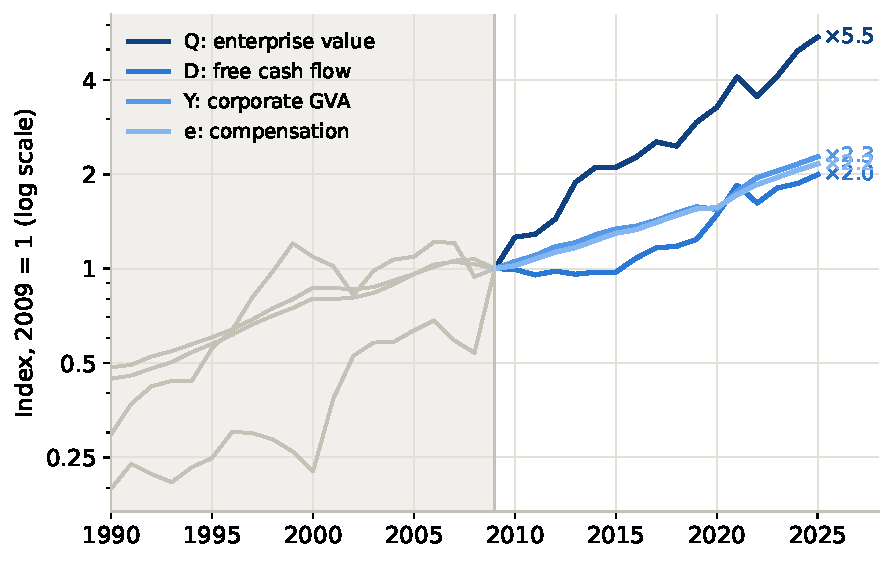
\includegraphics[width=\linewidth]{figures/f01_multiples.pdf}
\column{0.44\textwidth}
{\small
\begin{tabular}{@{}lrrrr@{}}\toprule
 & \multicolumn{2}{c}{2009 到 2025} & \multicolumn{2}{c}{2011 到 2025}\\
 & 倍数 & 年增速 & 倍数 & 年增速\\\midrule
$Q$ & $\times\val{multQ}$ & \val{grQ}\% & $\times\val{multBQ}$ & \val{grBQ}\%\\
$D$ & $\times\val{multFCF}$ & \val{grFCF}\% & $\times\val{multBFCF}$ & \val{grBFCF}\%\\
$Y$ & $\times\val{multY}$ & \val{grY}\% & $\times\val{multBY}$ & \val{grBY}\%\\
$e$ & $\times\val{multCOMP}$ & \val{grCOMP}\% & $\times\val{multBCOMP}$ & \val{grBCOMP}\%\\\bottomrule
\end{tabular}}\\[0.3cm]
{\small Theorem 1 条件 (i) 要求 $g_e>g_D$。以 2009 为基年 $g_D-g_e=\val{gapDe09}$ 个百分点/年，以 2011 为基年 $+\val{gapDe11}$：差异全部来自 2009 年的 FCF 高峰（净资本形成为负）。没有任何窗口给出 $D/e\to0$ 所需的持续负差。靠 ``$D$ 相对储蓄基数缩小'' 的机制，包括 $\varphi\to0$、$\rho>1$ 的份额漂移、Hirano–Toda (2023) 式的固定要素份额下降，在窗口内没有可匹配的对象。}
\end{columns}
\src{\texttt{2\_Check/figures/figure\_data.csv}：AHP 总公司部门口径，名义值。灰色为 2009 之前。}
\end{frame}

% ---------------------------------------------------------------- 5
\begin{frame}{数据事实 2：收益率下降发生在 $Q$，不在 $D$}{The yield fell through valuation}
\centerline{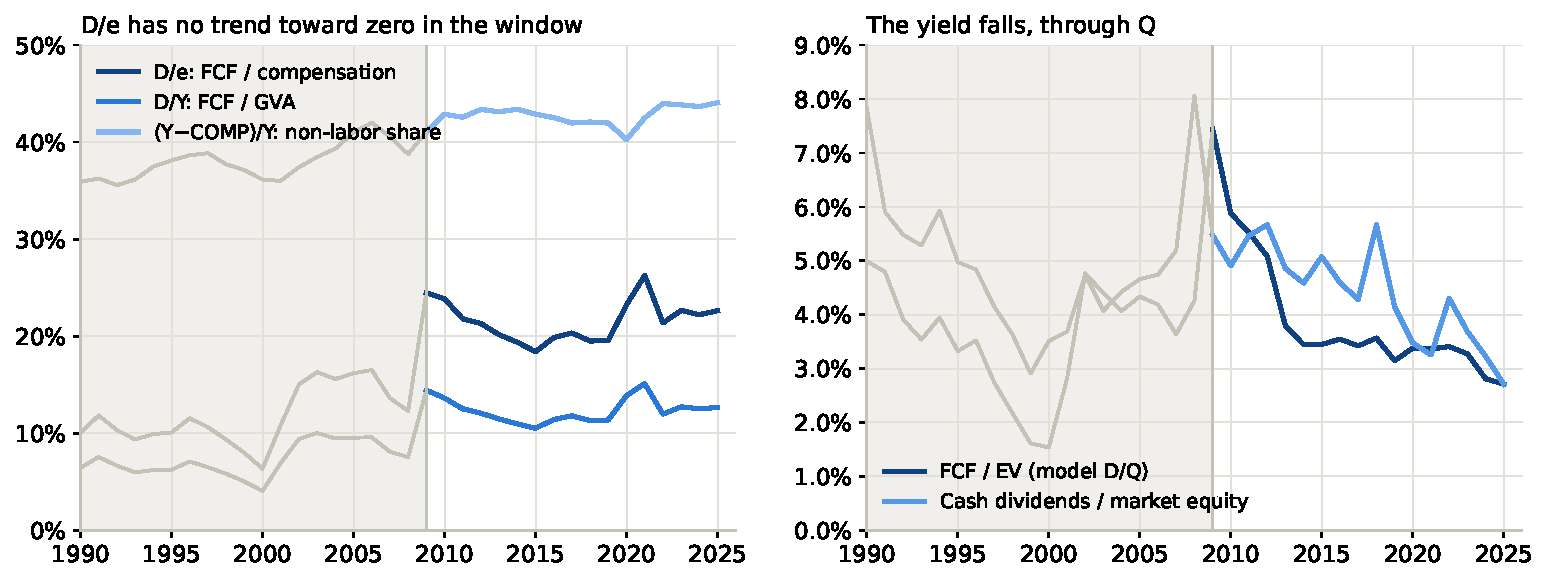
\includegraphics[width=0.7\textwidth]{figures/f02_de_dq.pdf}}
\begin{columns}[T]
\column{0.5\textwidth}
{\footnotesize
\begin{tabular}{@{}lrrrr@{}}\toprule
 & 2009 & 2011 & 2013 & 2025\\\midrule
$D/Q$ \en{(FCF/EV)} & \val{D_Q2009}\% & \val{D_Q2011}\% & \val{D_Q2013}\% & \val{D_Q2025}\%\\
现金股息/股权市值 & \val{CASHDIV_EQ2009}\% & \val{CASHDIV_EQ2011}\% & \val{CASHDIV_EQ2013}\% & \val{CASHDIV_EQ2025}\%\\
$D/e$ & \val{D_e2009}\% & \val{D_e2011}\% & \val{D_e2013}\% & \val{D_e2025}\%\\
$Q/e$ & \val{Q_e2009} & \val{Q_e2011} & \val{Q_e2013} & \val{Q_e2025}\\
隐含 $\beta$ & \val{A_e2009} & \val{A_e2011} & \val{A_e2013} & \val{A_e2025}\\\bottomrule
\end{tabular}}
\column{0.47\textwidth}
{\footnotesize $D/e$ 从 2009 年的高点回落后在 18\% 到 23\% 之间波动；$Q/e$ 升了 2.5 倍。收益率的下降有 2009 到 2012 的危机后高峰，之后从约 3.5\% 缓降到 2.7\%。现金股息口径降得更多（回购替代股息，Fama–French 2001），但现金股息仍与 $e$ 同速。}
\end{columns}
\src{现金股息收益率：Fed Z.1 总股息/股权市值，\texttt{Mechanism\_Evidence\_US\_ROW/processed/corporate\_yields.csv}。}
\end{frame}

% ---------------------------------------------------------------- 6
\begin{frame}{分解：$\Delta\log(Q/D)=\Delta\log(Q/Y)-\Delta\log(D/Y)$}{The model gets the channel backwards}
\begin{columns}[T]
\column{0.6\textwidth}
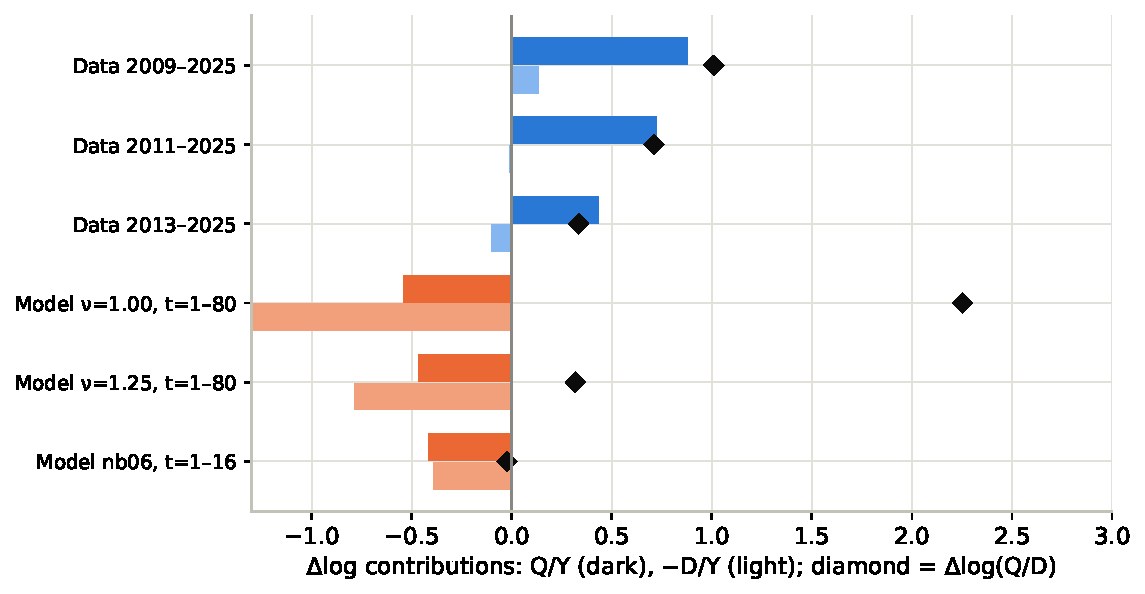
\includegraphics[width=0.95\linewidth]{figures/f03_decomp.pdf}
\column{0.38\textwidth}
{\small 2009 起 $Q/Y$ 贡献 \val{decShare2009}\%，其余是 2009 年 FCF 高峰的回落；2011 起 $Q/Y$ 贡献 \val{decShare2011}\%，$D/Y$ 持平；2013 起 $D/Y$ 上升，$Q/Y$ 贡献超过全部。\\[0.3cm]
模型三条路径的分解方向相反：$Q/Y$ 下降，$D/Y$ 坍缩。这是 memo 第 4 行 ``wrong channel'' 的图示。}
\end{columns}
\src{数据窗口由 \texttt{figure\_data.csv} 直接计算；模型为 AHP 种子 $\nu_u\in\{1,1.25\}$ 到 $T=80$ 与 notebook 06 最优点（\texttt{slides/data/decomp\_model.csv}）。}
\end{frame}

% ---------------------------------------------------------------- 7
\begin{frame}{R\&D share：数据 3 到 10\%，模型趋于 1}{The share that would have to carry the mechanism}
\centerline{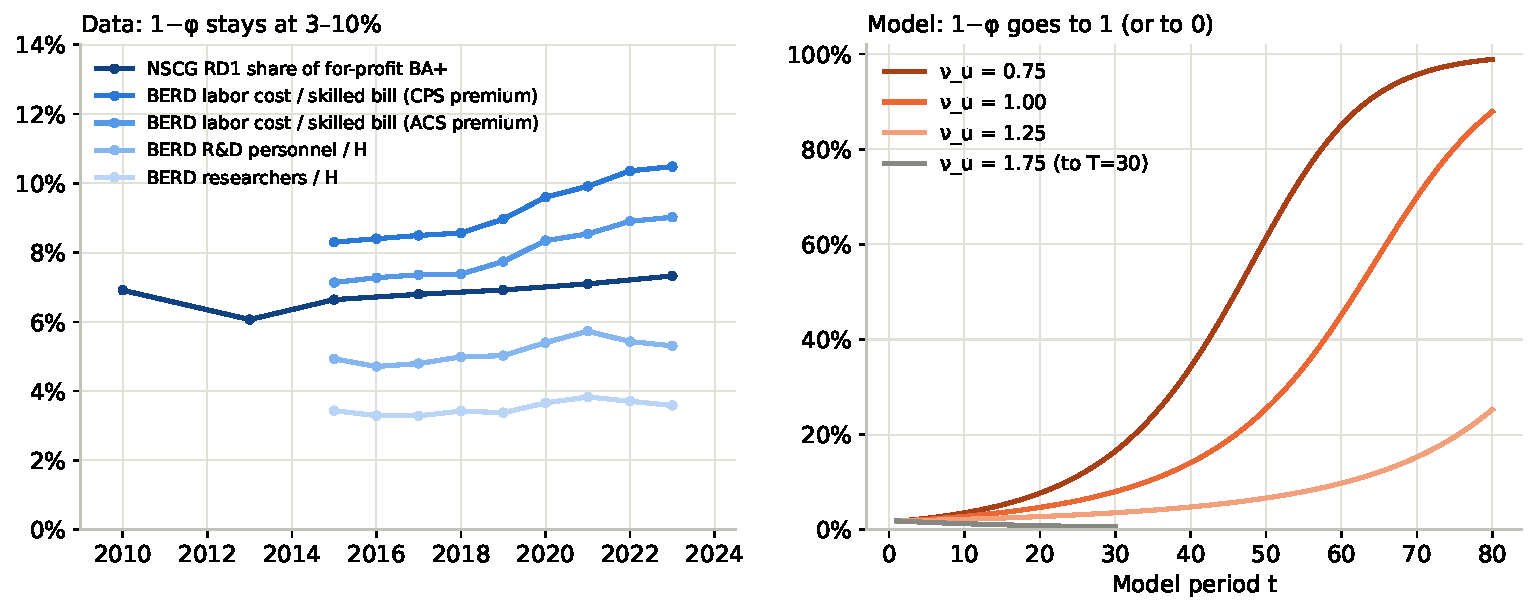
\includegraphics[width=0.8\textwidth]{figures/f06_rd_share.pdf}}
{\footnotesize NSCG RD1 份额 \val{nscg2010}\%（2010）到 \val{nscg2023}\%（2023）；BERD 人工成本/技能工资总额 \val{lccps2015}\%（2015）到 \val{lccps2023}\%（2023，CPS 溢价）；BERD 研究人员/$H$ 约 3.5\%。十年约 +1 到 2 个百分点。模型在 $\nu_u\le1.25$ 下 $1-\varphi$ 趋于 0.25 到 0.99，在 $\nu_u=1.75$ 下趋于 0。}
\src{\texttt{Skill\_Premium\_and\_RD\_Share\_2026-10-26}；模型扫描 \texttt{outputs\_zero\_nu\_b/05}。}
\end{frame}

% ---------------------------------------------------------------- 8
\begin{frame}{收益率恒等式：同一条下降，两种读法，且取决于基年}{The yield identity inside the free-entry block}
用知识法则 $G-1=a(1-\varphi)H$ 消去 $a$，并记 $\mu=1/\vartheta$，aggregate yield 为
\[
\frac{D}{Q}=\frac{N_t}{N_{t+1}}\frac{d}{q}=(\mu-1)\cdot\frac{\varphi}{1-\varphi}\cdot\frac{G-1}{G}.
\]
\begin{columns}[T]
\column{0.47\textwidth}
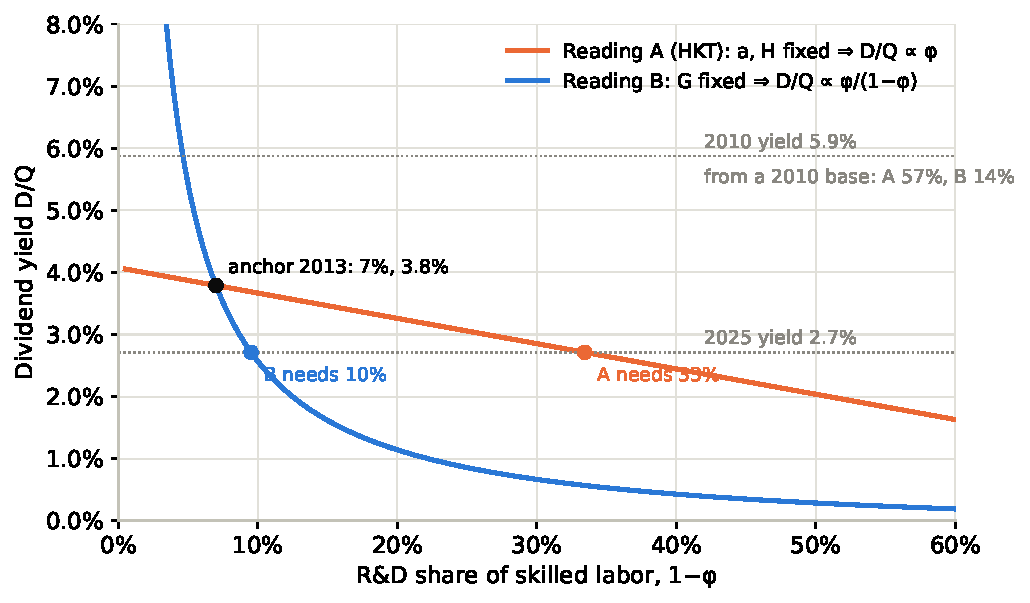
\includegraphics[width=\linewidth]{figures/f09_yield_identity.pdf}
\column{0.51\textwidth}
{\scriptsize 匹配 2025 年收益率 \val{D_Q2025}\% 所需的 $1-\varphi$，基年份额取 7\%：\\[0.05cm]
\begin{tabular}{@{}lrrr@{}}\toprule
基年 & 基年收益率 & 读法 A（固定 $a,H$） & 读法 B（固定 $G$）\\\midrule
2009 & \val{D_Q2009}\% & \val{reqA2009}\% & \val{reqB2009}\%\\
2010 & \val{D_Q2010}\% & \val{reqA2010}\% & \val{reqB2010}\%\\
2011 & \val{D_Q2011}\% & \val{reqA2011}\% & \val{reqB2011}\%\\
2013 & \val{D_Q2013}\% & \val{reqA2013}\% & \val{reqB2013}\%\\
2015 & \val{D_Q2015}\% & \val{reqA2015}\% & \val{reqB2015}\%\\\bottomrule
\end{tabular}\\[0.2cm]
读法 A 是 HKT 的 $D/Q\propto\varphi$，任何基年都需要 27\% 以上。读法 B 的弹性是 $1/(1-\varphi)$：从危机后高峰（2010、2011）起算需要翻倍到 13 到 14\%，超过观测的 7 到 10.5\%；从 2013 或 2015 起算只需 9\%，与 BERD 人工成本份额的上升一致。窗口内收益率的下降一部分是 2009 到 2012 高峰的回落，其余读法 B 能解释，读法 A 不能。}
\end{columns}
\end{frame}

% ---------------------------------------------------------------- 9
\begin{frame}{水平能对上：自由进入隐含的知识增速与加成}{Levels are consistent at a slow knowledge clock}
\begin{columns}[T]
\column{0.5\textwidth}
{\small 自由进入给出 $Q=w_H/a+I$，$I=(1-\varphi)B_H$，故
\[
G-1=\frac{I}{Q-I},\qquad \mu=1+\frac{D/Q}{\frac{1-\varphi}{\varphi}\cdot\frac{G-1}{G}} .
\]
\begin{tabular}{@{}lrrr@{}}\toprule
$1-\varphi=7\%$ & $B_H/Q$ & $G-1$ & 隐含 $\mu$\\\midrule
2010 & \val{BHQ2010} & \val{G07_2010}\% & \val{mu07_2010}\\
2013 & \val{BHQ2013} & \val{G07_2013}\% & \val{mu07_2013}\\
2015 & \val{BHQ2015} & \val{G07_2015}\% & \val{mu07_2015}\\
2019 & \val{BHQ2019} & \val{G07_2019}\% & \val{mu07_2019}\\
2022 & \val{BHQ2022} & \val{G07_2022}\% & \val{mu07_2022}\\
2024 & \val{BHQ2024} & \val{G07_2024}\% & \val{mu07_2024}\\\bottomrule
\end{tabular}}
\column{0.48\textwidth}
{\small
\begin{itemize}\setlength{\itemsep}{0.2cm}
\item 2013 到 2024 年，$1-\varphi\in\{5,7,10\}\%$ 下知识增速 $G-1$ 落在 \val{Gmin}\% 到 \val{Gmax}\%/年，隐含 $\mu$ 落在 \val{mumin} 到 \val{mumax}。
\item 这与扣除资本后的 P1 加成 1.45 到 1.73、De Loecker–Eeckhout–Unger (2020) 的 1.61 在同一区间。
\item R1 条件拟合里 22 到 30\% 的 R\&D share 是 $\mu=3.5$ 加无资本假设的产物，不是 block 的要求。
\item 代价：知识增速只有约 0.5\%/年，接近 TFP 增速而不是 R\&D 资本存量的 3\%。
\end{itemize}}
\end{columns}
\src{\texttt{data/t7\_free\_entry\_levels.csv}；$B_H$ 用 CPS 重新截尾溢价桥接，$D$ 为 AHP FCF。}
\end{frame}

% ---------------------------------------------------------------- 10
\begin{frame}{趋势对不上：常数 $a$ 被否定，隐含 $a$ 的下降比 BJVW 还陡}{Fishing out: the one within-block fix the data support}
\centerline{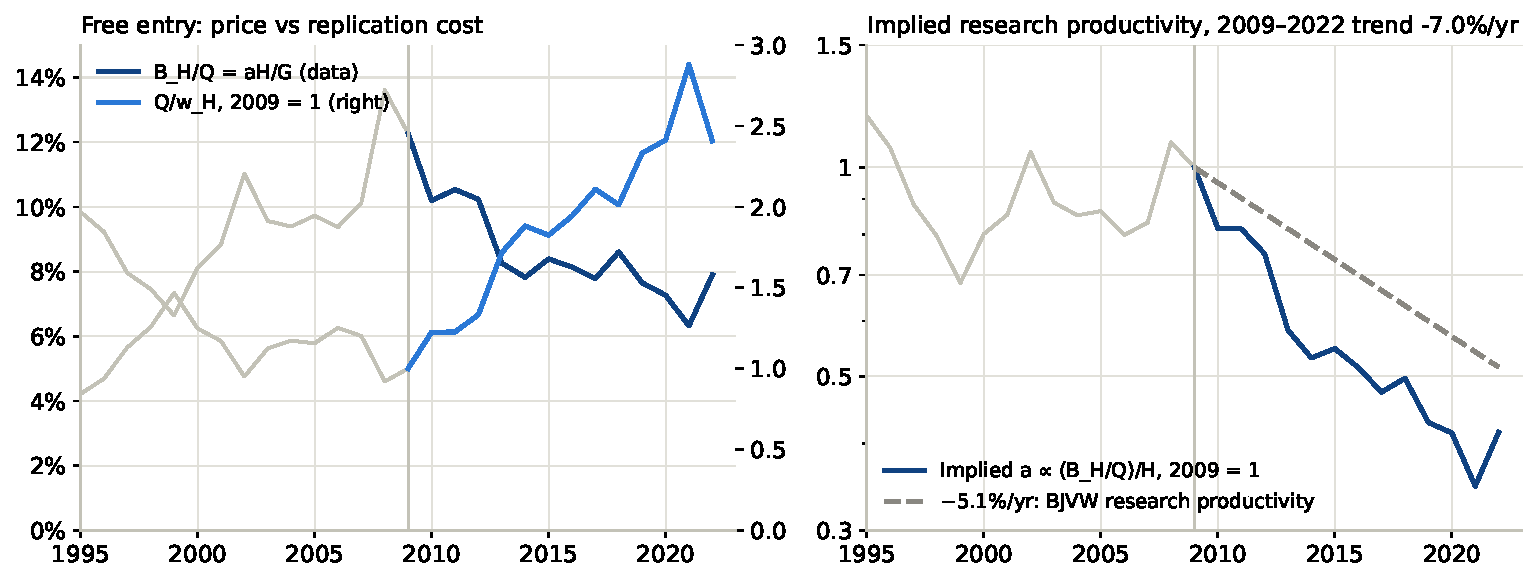
\includegraphics[width=0.84\textwidth]{figures/f05_free_entry.pdf}}
{\footnotesize $B_H/Q=aH/G$。2009 到 2024 年 $H$ 每年 +\val{Hgr}\%（$\times\val{Hmult}$），$B_H/Q$ 却从 \val{BHQ2009} 降到 \val{BHQ2022}，$Q/w_H$ 升至 \val{QwH0922} 倍。隐含 $a$ 在 2009 到 2022 年的趋势为 \val{aSlope}\%/年，2022 年只剩 2009 年的 \val{aIdx2022}；Bloom–Jones–Van Reenen–Webb (2020) 估计总量研究生产率 $-5.1\%$/年、研究投入 +4.3\%/年。半内生增长 \en{(Jones 1995)} 的 $a_t\downarrow$ 同时解释 $Q/w_H\uparrow$、$B_H/Q\downarrow$ 和 $(1-\varphi)H$ 每年 +4\% 而 $G$ 不变。但在 BGP 上 $a_tH_t$ 为常数，收益率也是常数：$a_t\downarrow$ 不能单独制造 explosive P/D。}
\end{frame}

% ---------------------------------------------------------------- 11
\begin{frame}{机制 1 与 2：资金来源不是一代人的工资}{Funding side: world savings and the wealth stock}
\centerline{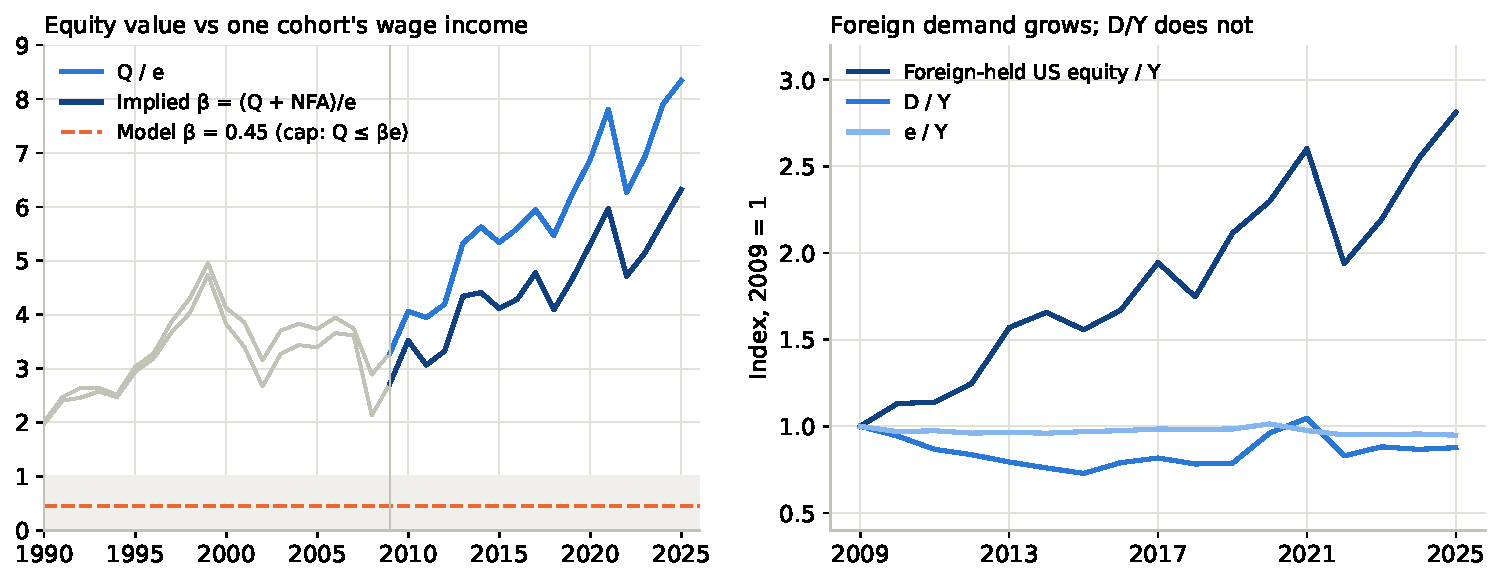
\includegraphics[width=0.7\textwidth]{figures/f04_funding.pdf}}
\begin{columns}[T]
\column{0.49\textwidth}
{\footnotesize \textbf{世界储蓄。} 外资持有美国股权/$Y$ 从 \val{EL_Y_sept2009} 升到 \val{EL_Y_sept2025}（$\times\val{ELYmult}$，2009 到 2025；2011 起 $\times\val{ELYmult11}$），$D/Y$ 同期 $\times\val{DYmult}$（2011 起 $\times\val{DYmult11}$）；2025 年外资约占 EV 的 42\%。Hirano–Toda (2025) necessity 的逻辑 ``储蓄基数增长快于 $D$'' 在这个口径下成立。模型里对应 $Q_{US}\le\beta e_{US}+s_We_W\bar\omega^*$，$e_W\approx3e_{US}$。CFG (2008)；AHP (2022)。}
\column{0.49\textwidth}
{\footnotesize \textbf{财富存量。} 外资只占 42\%，国内部分仍约 $3.7e$，超过任何 $\beta<1$。需要多期生命、遗赠或财富集中，让 $Q$ 由财富存量融资。Piketty–Zucman (2014) 财富/收入比约 3 升到 5 至 6；Auclert 等 (2021)；Mian–Straub–Sufi (2020)；Rachel–Summers (2019) 中性利率降约 3 个百分点。目标矩：隐含 $\beta$ 从 \val{A_e2009} 到 \val{A_e2025}。}
\end{columns}
\end{frame}

% ---------------------------------------------------------------- 12
\begin{frame}{机制 3：股票供给收缩，需求无弹性}{Supply of claims: the wrong supply curve in the model}
\centerline{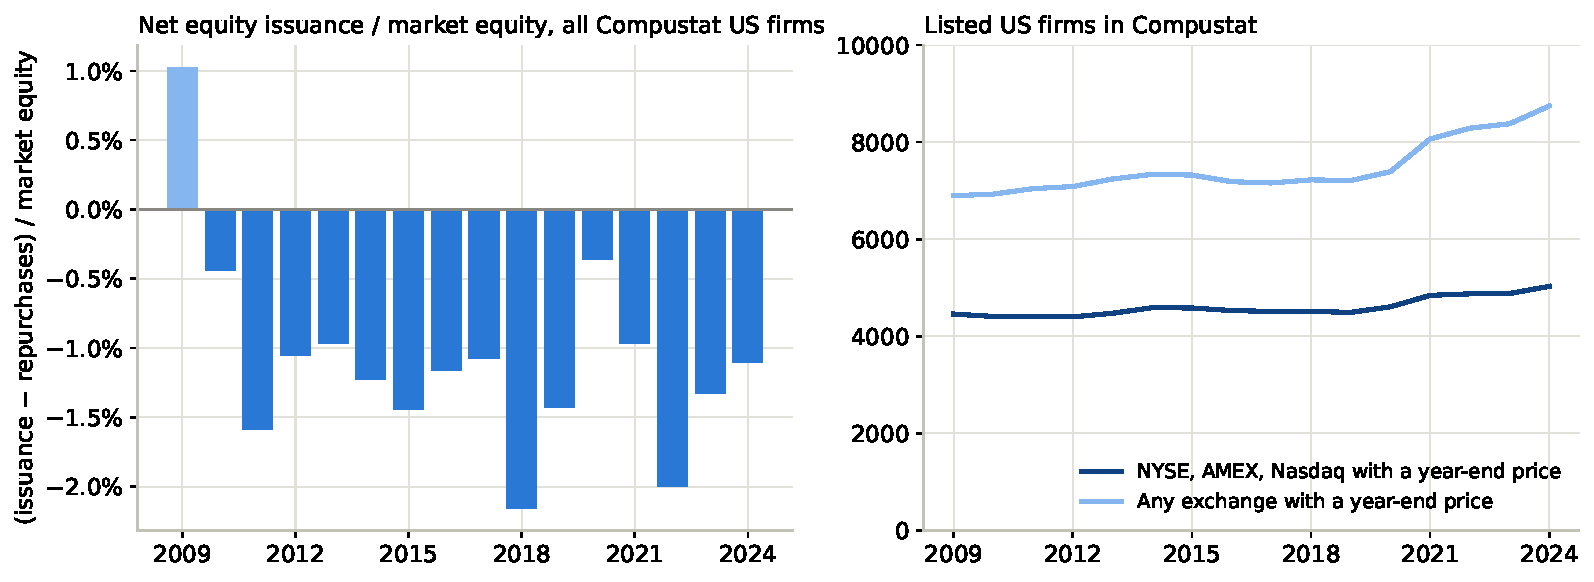
\includegraphics[width=0.7\textwidth]{figures/f08_supply.pdf}}
{\footnotesize Compustat 美国公司合计，2009 到 2024 年：净发行（发行减回购）/市值年均 \val{netissMean}\%，\val{netissYears} 年中 \val{netissNegYears} 年为负；累计回购 \val{buybackCum} 万亿美元对发行 \val{issueCum} 万亿；2024 年回购 \val{buyback2024} 对发行 \val{issue2024}（十亿美元）。NYSE/AMEX/Nasdaq 上市公司数 2009 年 \val{allNlisted2009}，2012 年低点 \val{allNlistedMin}，2024 年 \val{allNlisted2024}（含 SPAC；CRSP 口径自 1996 年减半见 Doidge–Karolyi–Stulz 2017）。Gabaix–Koijen (2021)：1 美元流入推高市值约 5 美元；Kuvshinov–Zimmermann (2022)：市值/GDP 的 ``大爆炸'' 几乎全是价格，净发行占比平稳。模型的自由进入是 $w_H/(aN)$ 处完全弹性的供给曲线，数据里供给在收缩：需要凸进入成本、有限进入或不可复制的租金。}
\end{frame}

% ---------------------------------------------------------------- 13
\begin{frame}{机制 4：租金与无形资本抬高 $D$ 和 $Q$，不是 P/D}{Rents explain why $D/Y$ did not fall}
\begin{columns}[T]
\column{0.56\textwidth}
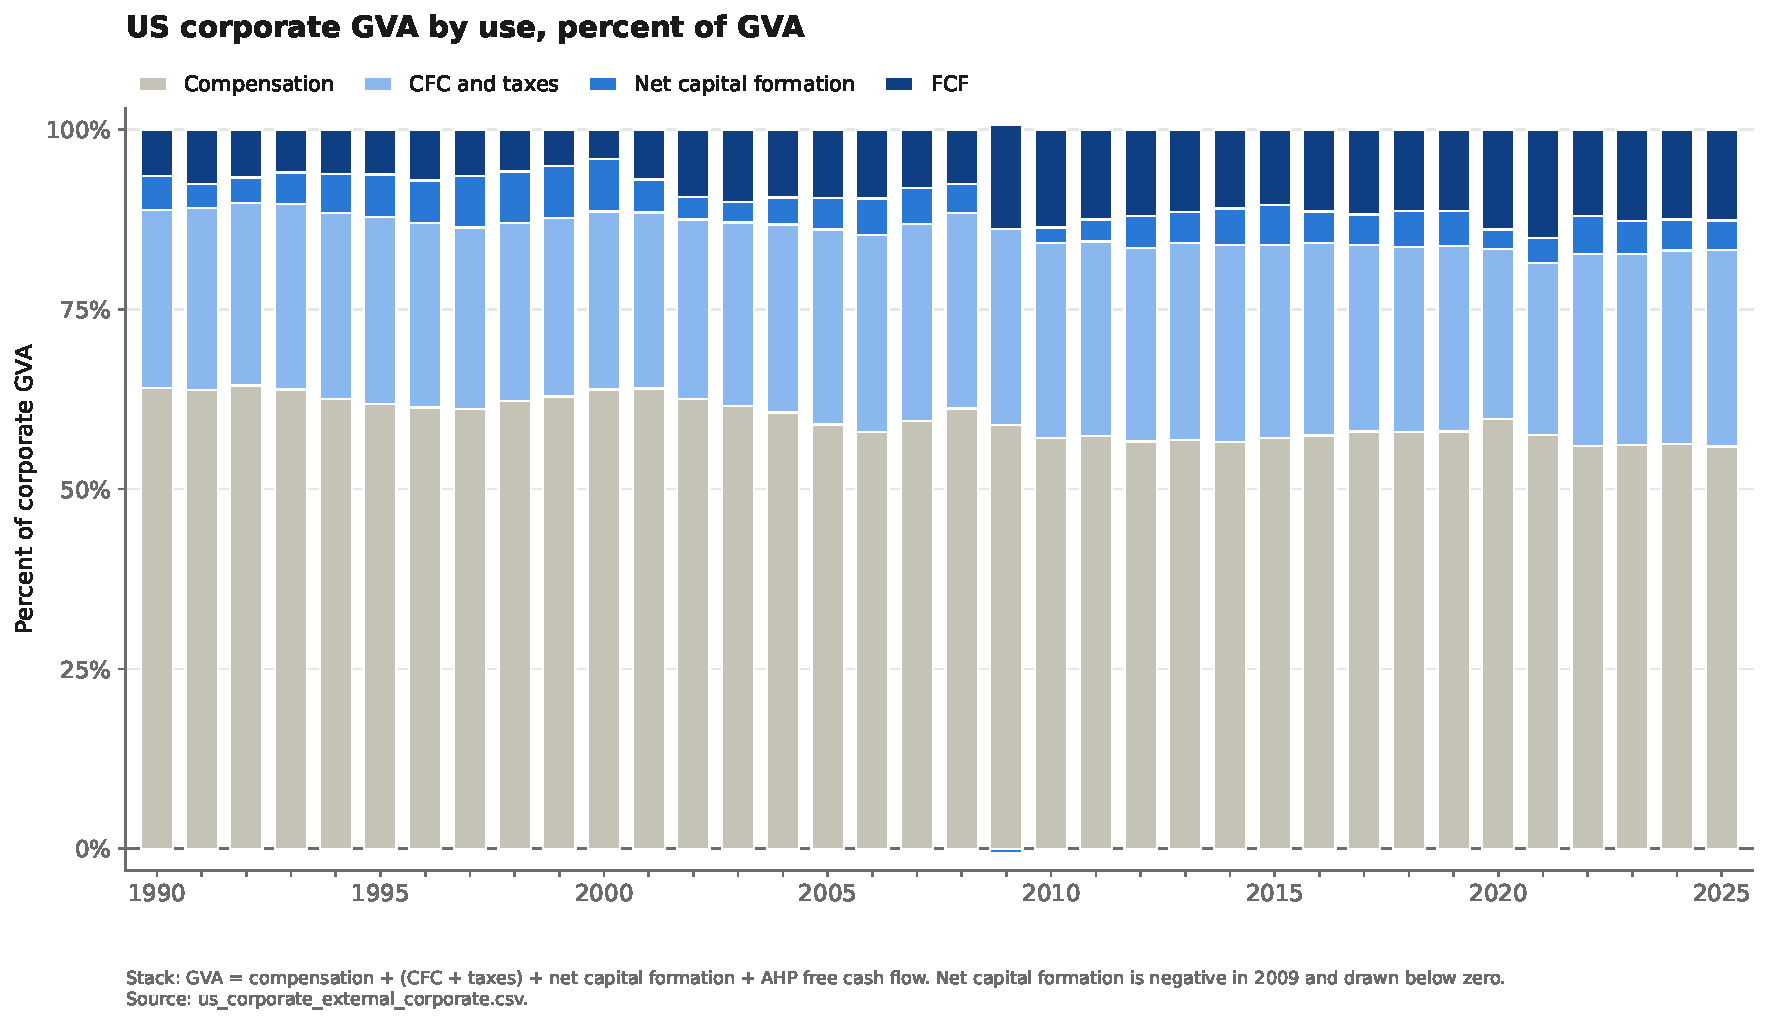
\includegraphics[width=0.96\linewidth]{../figures/gva_decomposition_percent_1990_2025.pdf}
\column{0.42\textwidth}
{\footnotesize 窗口内非劳动份额 $(Y-\mathrm{COMP})/Y$ 从 \val{PROFIT_SHARE2009}\% 升到 \val{PROFIT_SHARE2025}\%，FCF/$Y$ 在 \val{D_Y2025}\% 附近，都停在危机前已经达到的高位（图中 1990 到 2008 为背景）。\\[0.25cm]
Greenwald–Lettau–Ludvigson (2025)：1989 到 2017 年股权增值约四成来自向股东的再分配，约三分之一来自折现率下降，约四分之一来自增长（比例随版本略变）。De Loecker–Eeckhout–Unger (2020) 加成 1.21 到 1.61；Barkai (2020)；Eggertsson–Robbins–Wold (2021)；Farhi–Gourinchas (2018)；Crouzet–Eberly (2023)。\\[0.25cm]
含义：窗口内 $D/Y$ 高而平，是租金而非 R\&D 进入成本吸收了劳动份额的下降。这正是 HKT 通道失效的原因，也是模型需要资本与租金的原因（memo 第 3 节第 2 条）。}
\end{columns}
\end{frame}

% ---------------------------------------------------------------- 14
\begin{frame}{检验设计：在位企业队列}{Can the dividend collapse survive at the firm level?}
\begin{columns}[T]
\column{0.5\textwidth}
{\small \textbf{假说。} HKT 的分红坍缩是 per-variety 的：新品种稀释在位品种的 $d_t\propto w_H\varphi H/N_t$。总量 $D$ 不降，但一组固定的在位企业的股息可能增长慢于 $e$（创造性破坏版）。\\[0.25cm]
\textbf{检验。} 取 $t_0\in\{2009,2010,2011\}$ 年有正总资产的美国公司（Compustat 年度基本面，\texttt{indfmt=INDL, consol=C, fic=USA}），固定集合，逐年加总仍在报告的成员：
\[
D^{\mathrm{coh}}_t=\sum_{i\in\mathcal C_{t_0}}\mathrm{dvt}_{it},\quad
\mathrm{NP}^{\mathrm{coh}}_t=\sum(\mathrm{dvt}+\mathrm{prstkc}-\mathrm{sstk})_{it},
\]
再比较 $g(D^{\mathrm{coh}})$ 与 $g(e)$。H$_0$（HKT 企业层面）：$g(D^{\mathrm{coh}})<g(e)$。}
\column{0.48\textwidth}
{\small \textbf{口径。} 现金股息 \en{(dvt)}、净 payout（股息加回购减发行）、FCF（经营现金流减资本支出）、市值 \en{(csho$\times$prcc\_f)}。名义值，与 AHP 的 $e$ 同币种同频率。\\[0.25cm]
\textbf{已知偏差。} 队列随并购与退市收缩（2009 队列 \val{c2009n0} 家到 2024 年 \val{c2009n2024} 家）。被队列外企业并购的成员，其品种的股息从队列中消失，使队列股息向下偏，即对 H$_0$ 有利。2009 年回购几乎停止、发行高企，所以 2009 基年的净 payout 增速被起点压低而放大；2011 基年是干净的对照。\\[0.25cm]
\textbf{数据。} 31.8 万条企业年观测，1989 到 2024 财年，2026-11-13 直连 WRDS 提取（\texttt{data/wrds/manifest.json}）。}
\end{columns}
\end{frame}

% ---------------------------------------------------------------- 15
\begin{frame}{检验结果：在位企业的股息快于 $e$，价格快得多}{H$_0$ is rejected: no firm-level dividend collapse either}
\centerline{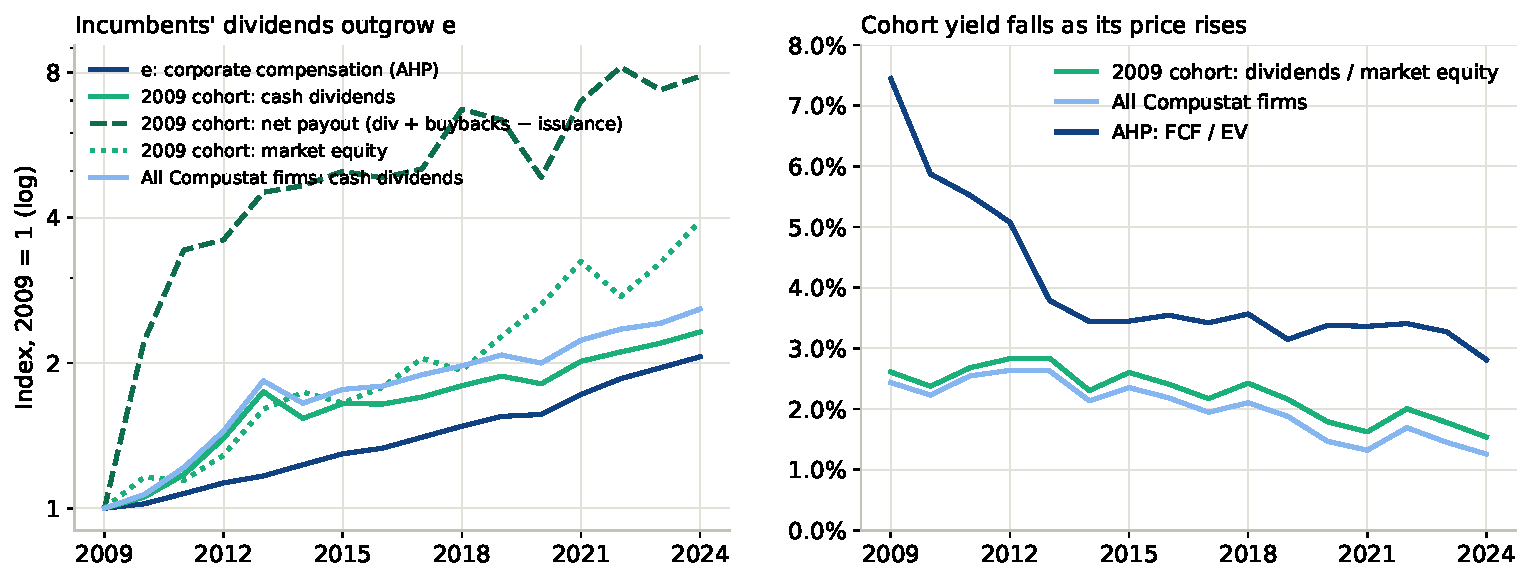
\includegraphics[width=0.86\textwidth]{figures/f07_cohort.pdf}}
{\footnotesize 2009 队列（\val{c2009n0} 家）到 2024 年：现金股息 $\times\val{c2009dvt_mult}$（\val{c2009dvt_gr}\%/年）对 $e$ 的 $\times\val{c2009comp_mult}$（\val{c2009comp_gr}\%/年）；净 payout $\times\val{c2009netpay_mult}$（2009 起点被危机压低，2011 队列为 $\times\val{c2011netpay_mult}$）；FCF $\times\val{c2009fcf_mult}$（2009 起点被压高）；队列市值 $\times\val{c2009me_mult}$（\val{c2009me_gr}\%/年）。队列股息收益率从 \val{c2009dvt_me0}\% 降到 \val{c2009dvt_me2024}\%。即便队列向下偏，股息增速仍高于 $e$；队列 P/D 的上升同样是 $Q$ 的现象：价格增速接近股息增速的两倍。}
\end{frame}

% ---------------------------------------------------------------- 16
\begin{frame}{稳健性：2010 与 2011 队列，以及队列份额}{Later bases and what exits do}
\centerline{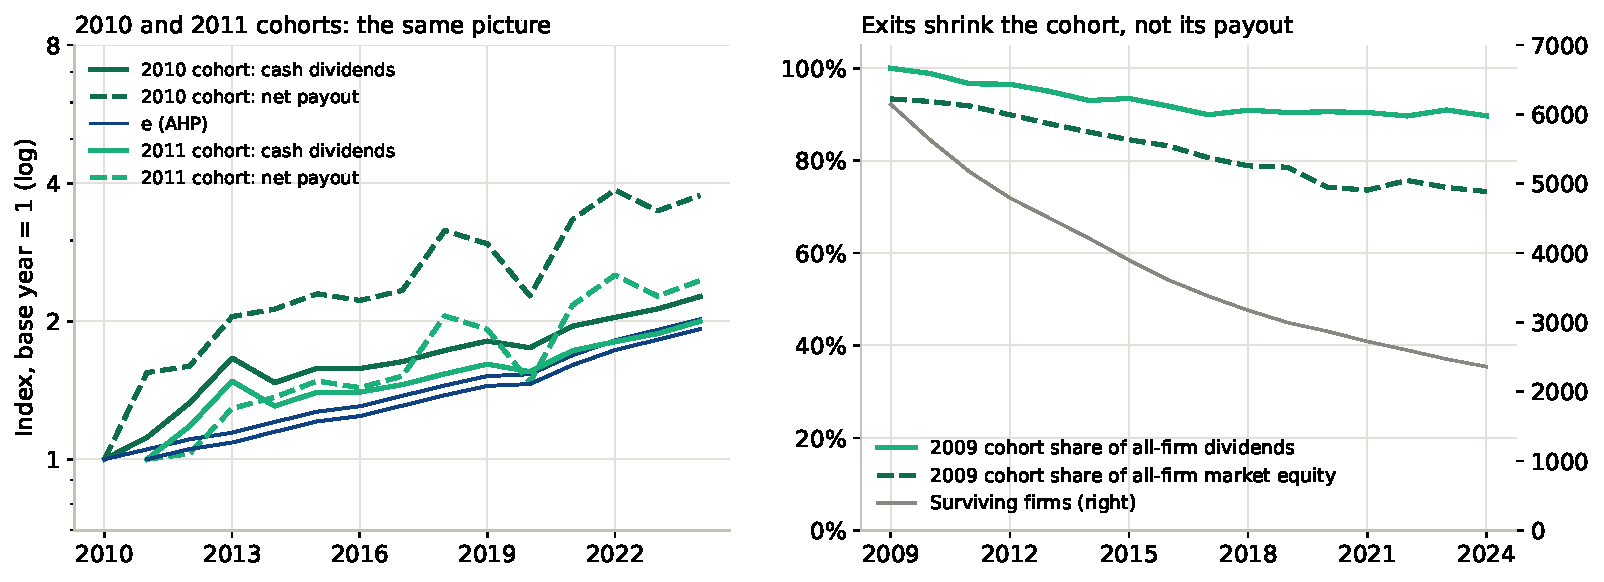
\includegraphics[width=0.74\textwidth]{figures/f07b_cohort_more.pdf}}
{\scriptsize
\begin{tabular}{@{}lrrrrrrr@{}}\toprule
队列（到 2024） & 家数 & 现金股息 & 净 payout & 市值 & $e$ & 占全部股息 & 占全部市值\\\midrule
2009 & \val{c2009n0} $\to$ \val{c2009n2024} & $\times$\val{c2009dvt_mult} & $\times$\val{c2009netpay_mult} & $\times$\val{c2009me_mult} & $\times$\val{c2009comp_mult} & \val{c2009share_dvt2024}\% & \val{c2009share_me2024}\%\\
2010 & \val{c2010n0} $\to$ \val{c2010n2024} & $\times$\val{c2010dvt_mult} & $\times$\val{c2010netpay_mult} & $\times$\val{c2010me_mult} & $\times$\val{c2010comp_mult} & \val{c2010share_dvt2024}\% & \val{c2010share_me2024}\%\\
2011 & \val{c2011n0} $\to$ \val{c2011n2024} & $\times$\val{c2011dvt_mult} & $\times$\val{c2011netpay_mult} & $\times$\val{c2011me_mult} & $\times$\val{c2011comp_mult} & \val{c2011share_dvt2024}\% & \val{c2011share_me2024}\%\\\bottomrule
\end{tabular}}\\[0.2cm]
{\footnotesize 三个队列的现金股息都快于 $e$，净 payout 更快。退出使队列家数降到 38 到 43\%，但 2009 队列仍发放全部 Compustat 股息的 \val{c2009share_dvt2024}\%，而只占市值的 \val{c2009share_me2024}\%：新进入者稀释的是市值份额，不是股息。这与 HKT 的 ``新品种分走在位者的 $d$'' 相反：新品种分走的是 $Q$。}
\end{frame}

% ---------------------------------------------------------------- 17
\begin{frame}{替代机制的排序}{Ranking by what the 2009–2025 data can discipline}
{\scriptsize
\renewcommand{\arraystretch}{1.3}
\begin{tabular}{@{}>{\raggedright\arraybackslash}p{0.17\textwidth}>{\raggedright\arraybackslash}p{0.29\textwidth}>{\raggedright\arraybackslash}p{0.26\textwidth}>{\raggedright\arraybackslash}p{0.23\textwidth}@{}}\toprule
机制 & 2009 到 2025 年的证据 & 外部证据 & 能否 explosive\\\midrule
1. 世界储蓄 \en{(foreign demand)} & 外资持有/$Y$ $\times\val{ELYmult}$ 对 $D/Y$ $\times\val{DYmult}$；42\% 的 EV & CFG 2008；AHP 2022 & 能，若 RoW 储蓄对美股的配置持续快于 $D$\\
2. 财富存量 \en{(wealth stock)} & 隐含 $\beta$ \val{A_e2009} 到 \val{A_e2025} & Piketty–Zucman 2014；Auclert 等 2021；MSS 2020；Rachel–Summers 2019 & 能，若财富/收入持续上升\\
3. 供给收缩与无弹性需求 & 净发行年均 \val{netissMean}\% 市值；$Q/w_H$ $\times$\val{QwH0922}；$B_H/Q\downarrow$ & Gabaix–Koijen 2021；DKS 2017；KZ 2022 & 放大 1、2，本身有界\\
4. 租金与无形资本 & 非劳动份额 \val{PROFIT_SHARE2009} 到 \val{PROFIT_SHARE2025}\%，高而平 & GLL 2025；DLEU 2020；ERW 2021；FG 2018；CE 2023 & 否：抬高 $D$，份额有界\\
5. 研究生产率下降 \en{(fishing out)} & 隐含 $a$ 趋势 \val{aSlope}\%/年 & BJVW 2020；Jones 1995, 2022 & 否（BGP 上收益率常数）；修复 $Q/w_H$ 与 $B_H/Q$ 的趋势\\
0. R\&D share $\to1$（现有） & $1-\varphi$ 3 到 10\%，$D/e$ 无趋势，队列股息快于 $e$ & & 需要 $D/e\to0$：被总量与企业层面同时否定\\\bottomrule
\end{tabular}}
\end{frame}

% ---------------------------------------------------------------- 18
\begin{frame}{对模型的含义}{What to change, and which moments to target}
\begin{columns}[T]
\column{0.5\textwidth}
{\small
\begin{enumerate}\setlength{\itemsep}{0.22cm}
\item \textbf{资金侧。} 把 $\beta e$ 换成财富存量加世界储蓄：多期或 perpetual-youth 结构，$\bar\omega^*$ 上升。目标矩：隐含 $\beta$、股权负债/$Y$、AHP 估值效应。
\item \textbf{供给侧。} 用 $a_t\downarrow$（半内生）或凸进入成本替代常数 $a$。目标矩：$Q/w_H$ $\times$\val{QwH0922}、$B_H/Q$ 从 \val{BHQ2009} 到 \val{BHQ2022}。这同时解决 memo 第 6 行。
\item \textbf{$\rho>1$ 与 $\varphi$ 衰减降为次要通道。} 保留它只需 $1-\varphi$ 从 7\% 升到 9 到 14\%（取决于基年），不需趋于 1，也就不再要求 $\xi>\nu$ 去压 premium（memo 第 7 到 9 行）。
\item \textbf{加资本与租金。} 使 P1 在 $\mu\approx1.45$ 处可行，$D$ 的口径与 FCF 对齐。
\end{enumerate}}
\column{0.48\textwidth}
\begin{block}{necessity 条件的重写}
\small 若资金基数为 $W_t$（财富加外资配置），necessity 的条件变为 $g_W>g_D$ 与 $R<g_W$。2009 到 2025 年外资持有量/$Y$ 的 $\times\val{ELYmult}$ 对 $D/Y$ 的 $\times\val{DYmult}$ 满足前者；$r-g<0$ 在整个窗口满足后者。这是论文可以直接陈述的、与 $u$ 态数据相容的 necessity 版本。
\end{block}
\begin{block}{保留}
\small 2009 基年的 FCF 与 payout 起点有危机效应，故处处并报 2011 或 2013；知识存量增速 convention-driven；队列检验含并购偏差但偏向 H$_0$；Compustat 上市公司数口径与 CRSP 不同。
\end{block}
\end{columns}
\end{frame}

% ---------------------------------------------------------------- 19
\begin{frame}{附录：来源与口径}{Sources}
{\scriptsize
\textbf{窗口。} 主窗口 2009 到 2025 年（u 态）；1990 到 2008 只在图中以灰色显示。2009 年 FCF/$Y$ \val{D_Y2009}\%、$D/Q$ \val{D_Q2009}\% 为危机高峰，故并报 2011、2013 基年。\\[0.15cm]
\textbf{仓库数据。} \texttt{2\_Check/figures/figure\_data.csv}（AHP 总公司部门 $Y$、COMP、FCF、EV；CPS 桥接的 $B_H$）；\texttt{2\_Check/slides/data/}（\texttt{val\_us}, \texttt{vintage\_liab}, \texttt{free\_entry\_data}, \texttt{rd\_data}, \texttt{decomp\_model}, \texttt{sweep\_rd\_share*}）；\texttt{Empirical\_Mapping\_Annual/data\_intermediate/labor\_wages.csv}（$H$）；\texttt{Mechanism\_Evidence\_US\_ROW/processed/corporate\_yields.csv}（现金股息收益率）。外部头寸用 2026 年 9 月版。\\[0.15cm]
\textbf{Compustat。} \texttt{comp.funda} 1989 到 2024 财年，\texttt{indfmt=INDL, datafmt=STD, popsrc=D, consol=C, fic=USA, curcd=USD}；\texttt{comp.company} 的 SIC。重复的 gvkey-fyear 取总资产最大者。缺失的 dvt、prstkc、sstk、oancf、capx 记 0。队列：基年总资产大于 0。提取脚本 \texttt{scripts/fetch\_wrds.py}，清单 \texttt{data/wrds/manifest.json}。\\[0.15cm]
\textbf{文献。} Hirano–Kishi–Toda 2025 arXiv:2501.08215；Hirano–Toda 2025 JPE 10.1086/732528；Hirano–Toda 2023 arXiv:2307.00349；Bloom–Jones–Van Reenen–Webb 2020 AER 10.1257/aer.20180338；Jones 1995 JPE 10.1086/262002；Jones 2022 AER 10.1257/aer.20201605；Greenwald–Lettau–Ludvigson 2025 JPE 10.1086/734089；Kuvshinov–Zimmermann 2022 JFE 10.1016/j.jfineco.2021.09.008；Gabaix–Koijen 2021 NBER 28967；Doidge–Karolyi–Stulz 2017 JFE 10.1016/j.jfineco.2016.12.002；De Loecker–Eeckhout–Unger 2020 QJE 10.1093/qje/qjz041；Atkeson–Heathcote–Perri 2022 NBER 29771；Mian–Straub–Sufi 2020 NBER 26941；Auclert–Malmberg–Martenet–Rognlie 2021 NBER 29161；Rachel–Summers 2019 BPEA；Farhi–Gourinchas 2018 BPEA；Eggertsson–Robbins–Wold 2021 JME；Crouzet–Eberly 2023 JF；Barkai 2020 JF；Caballero–Farhi–Gourinchas 2008 AER；Piketty–Zucman 2014 QJE；Fama–French 2001 JFE。\\[0.15cm]
\textbf{重建。} \texttt{scripts/fetch\_wrds.py}（需 \texttt{\textasciitilde/.pgpass}），\texttt{scripts/build\_data.py}，然后 \texttt{latexmk -xelatex main.tex}。}
\end{frame}

\end{document}
